\documentclass{article}
% Input & Setup packages and commands needed
\usepackage{graphicx}
\usepackage{afterpage}
\usepackage{geometry}
\usepackage{float}
\usepackage[hidelinks]{hyperref}
\usepackage[perpage]{footmisc}
\usepackage{color}
\usepackage{listings}
\lstset{language=Go,
basicstyle=\ttfamily\scriptsize,
keywordstyle=\color{blue}\ttfamily,
stringstyle=\color{red}\ttfamily,
commentstyle=\color{green}\ttfamily}
\usepackage{xepersian}
\settextfont{XB Niloofar}

% configure paragraphs
\setlength{\parskip}{5pt}
\renewcommand{\baselinestretch}{1.8}


% configure un-ordered list settings

\renewcommand{\labelitemi}{$\bullet$}
\renewcommand{\labelitemii}{$\circ$}



\renewcommand{\bibname}{مراجع}

% Input data needed for titlepage from title.tex file
\title{
    \center
    
\includegraphics[width=5cm, height=5cm]{images/IUST_logo_color.png} \\ [10pt]
    دانشکده مهندسی کامپیوتر \\ [40pt]

    \textbf{ پیاده‌سازی درگاه ارتباط با رابط‌های برنامه‌نویسی} \\ [20pt]

    \textbf{ پایان‌نامه برای دریافت درجه‌ی کارشناسی در رشته‌ی مهندسی کامپیوتر} \\ [20pt]

}

\author{
    \textbf{میلاد ابراهیمی} \\ [30pt]


    \textbf{ استاد راهنما:} \\ [10pt]
    \textbf{دکتر وصال حکمی} \\ [10pt]
}



\date{
    شهریور ۱۳۹۹
}



\begin{document}

% title page with no numbering
\begin{titlepage}
    \clearpage\maketitle
    \thispagestyle{empty}
\end{titlepage}
\newpage\thispagestyle{empty}

% empty page
%\newpage\null\thispagestyle{empty}\newpage

\newpage
\thispagestyle{empty}
\begin{center}
    
\includegraphics[width=10cm]{images/besm.jpg}
\end{center}
\cleardoublepage

\newpage
\thispagestyle{empty}

\begin{center}
{\Large
    تأییدیه‌ی هیأت داوران جلسه‌ی دفاع از پایان‌نامه
}
\end{center}
\vspace{1cm}

نام دانشكده: مهندسی کامپیوتر

نام دانشجو: میلاد ابراهیمی

عنوان: پیاده‌سازی درگاه ارتباط با رابط‌های برنامه‌نویسی

تاریخ دفاع: شهریور ۱۳۹۹

رشته: مهندسی کامپیوتر \\[50pt]
\begin{center}
    \begin{tabular}{| p{8mm} | p{18mm} | p{.17\textwidth} |p{14mm}|p{.2\textwidth}|c|}
        \hline
        ردیف & سمت & نام و نام خانوادگی & مرتبه دانشگاهی & دانشگاه یا مؤسسه & امــضـــــــــا\\
        \hline
        ۱ & استاد راهنما & دکتر \newline وصال حکمی & استادیار & دانشگاه علم‌و‌صنعت ایران &    \\
        \hline
        ۲ & داور داخلی & دکتر \newline مهرداد آشتیانی & استادیار & دانشگاه علم‌و‌صنعت ایران   &     \\
        \hline


    \end{tabular}
\end{center}


\cleardoublepage 
\newpage
\thispagestyle{empty}

\begin{center}
{\Large
    تأییدیه‌ی صحت و اصالت نتایج \\
}
\vspace{.5cm}
باسمه تعالی
\vspace{.5cm}
\end{center}
%\doublespacing

اینجانب
سعید طهماسبی ثالث
به شماره دانشجویی
۹۵۵۲۱۳۱۵
دانشجوی رشته
مهندسی کامپیوتر
مقطع تحصیلی
کارشناسی
تأیید می‌نمایم كه كلیه‌ی نتایج این پایان‌نامه حاصل كار اینجانب و بدون هرگونه دخل و تصرف است و موارد نسخه‌برداری‌شده از آثار دیگران را با ذكر كامل مشخصات منبع ذكر كرده‌ام. درصورت اثبات خلاف مندرجات فوق، به تشخیص دانشگاه مطابق با ضوابط و مقررات حاكم (قانون حمایت از حقوق مؤلفان و مصنفان و قانون ترجمه و تكثیر كتب و نشریات و آثار صوتی، ضوابط و مقررات آموزشی، پژوهشی و انضباطی) با اینجانب رفتار خواهد شد و حق هرگونه اعتراض درخصوص احقاق حقوق مكتسب و تشخیص و تعیین تخلف و مجازات را از خویش سلب می‌نمایم. در ضمن، مسؤولیت هرگونه پاسخگویی به اشخاص اعم از حقیقی و حقوقی و مراجع ذی‌صلاح (اعم از اداری و قضایی) به عهده‌ی اینجانب خواهد بود و دانشگاه هیچ‌گونه مسؤولیتی در این خصوص نخواهد داشت.

\vspace{.5cm}
\begin{flushleft}
\begin{tabular}{lr}
نام و نام خانوادگی:   & 	سعید طهماسبی ثالث \\
تاریخ و امضا: & \\
\end{tabular}
\end{flushleft}
\cleardoublepage
\newpage
\thispagestyle{empty}
\begin{center}
{\Large
    مجوز بهره‌برداری از پایان‌نامه \\
}
    \vspace{.5cm}
\end{center}
%\doublespacing

بهره‌برداری از این پایان‌نامه در چهارچوب مقررات كتابخانه و با توجه به محدودیتی كه توسط استاد راهنما به شرح زیر تعیین می‌شود، بلامانع است:

\vspace{1cm}
\noindent$\Box$بهره‌برداری از این پایان‌نامه برای همگان بلامانع است.\\
$\Box$ بهره‌برداری از این پایان‌نامه با اخذ مجوز از استاد راهنما، بلامانع است.\\
$\Box$ بهره‌برداری از این پایان‌نامه تا تاریخ .................................... ممنوع است.\\

\vspace{1cm}
\begin{flushleft}
    \begin{tabular}{l p{.25\textwidth}}
        نام استاد راهنما: & دکتر وصال حکمی \\
        تاریخ: & \\
        امضا: & \\

    \end{tabular}
\end{flushleft}
\cleardoublepage
% change numbering style
\pagenumbering{harfi}


% input data of summary page
\section*{چکیده}
\addcontentsline{toc}{section}{\numberline{} چکیده‌}
با توجه به رشد روز‌افزون کسب و کارهای مجازی و نیاز به ثبات و کارایی بالا در تامین درخواست‌‌های مشتریان، معماری‌های جدیدی برای توسعه نرم‌افزار مورد استفاده قرار می‌گیرند. ویژگی اصلی این معماری‌ها، مقیاس‌مندی و تاب‌آوری بالا برای پاسخ به مشتریان است.

معماری میکروسرویس، یکی از محبوب‌ترین معماری‌های جدید است. تمرکز این معماری بر مقیاس‌مندی، گسترش‌پذیری و عدم وابستگی خدمت‌های مختلف یک سامانه به یکدیگر است. نحوه‌ی دستیابی این معماری به ویژگی‌های ذکر شده، جداسازی عملکرد‌های مختلف سامانه به چند قسمت و اجرای خودمختار هر یک از این قسمت‌ها در یک محیط جدا‌شده
\LTRfootnote{Isolated}
است.

همانند بسیاری از معماری‌های دیگر، پیاده‌سازی درست معماری میکروسرویس، دارای چالش‌های مختلفی است. با توجه به ماهیت غیر متمرکز سامانه‌ها در این معماری، اتصال کاربران به خدمت‌های ارائه‌شده به سادگی گذشته نخواهد بود. زیرا کاربر برای استفاده از خدمت‌های مختلف نیاز به دریافت اطلاعات از قسمت‌های مختلف سامانه را دارد. از طرفی تغییر روش ارتباط کاربران با سامانه و به‌روزرسانی نرم‌افزارهای سمت کاربر، بسیار پرهزینه خواهد بود.

الگوی درگاه ارتباط با رابط‌های برنامه‌نویسی جهت حل این چالش طراحی شده است. در این الگو، کاربران همانند سابق درخواست‌های خود را تنها به یک سامانه‌ی میانی ارسال می‌کنند. وظیفه‌ی این سامانه‌ی میانی، دریافت درخواست و هدایت ‌آن به سمت خدمت‌های مرتبط به درخواست است.

علی‌رغم وجود درگاه‌های ارتباط متن‌باز و تجاری مختلف، اکثر آن‌ها گسترش‌پذیری و قابلیت پیکربندی ضعیفی دارند. از این‌رو پیاده‌سازی یک درگاه ارتباط که خلاهای موجود را پوشش دهد، تمرکز اصلی این پروژه است.

\noindent {\bf کلید واژه‌ها:}
درگاه ارتباط با رابط‌های برنامه‌نویسی، معماری میکروسرویس، سامانه‌های غیر متمرکز، سامانه‌ی گسترش‌پذیر
\cleardoublepage 


% Set table of contents
\tableofcontents
\thispagestyle{empty}
\cleardoublepage

%Set table of figures
\listoffigures
%\addcontentsline{toc}{section}{\numberline{} فهرست تصاویر}
\cleardoublepage
%
%% Set table of tables
\listoftables
%\addcontentsline{toc}{section}{\numberline{} فهرست جداول}
\cleardoublepage

% reset page numbering to arabic
\pagenumbering{arabic}
\setcounter{page}{1}

\section{مقدمه}\label{sec:intro}

\subsection{تاریخچه}\label{subsec:intro_history}

گسترش روز‌افزون راه‌های ارتباطی از طریق شبکه و اینترنت، باعث ایجاد کسب‌وکار‌های بسیاری شده است. این فعالیت‌ها در حوزه‌های مختلفی از جمله درخواست خدمات حضوری، ارائه‌ی خدمات مجازی، شبکه‌های اجتماعی و ارتباطی و … انجام می‌شوند.

با توجه به محبوبیت روز‌افزون خدمات مجازی در بین مردم، کسب‌و‌کار‌ها نیز بزرگ و بزرگ‌تر می‌شوند. از این رو، ارائه‌ی خدمات مطمئن، سریع و با کیفیت مطلوب بخشی از اولویت‌های صاحبان کسب‌و‌کارهاست.

در ابتدای گسترش فناوری‌های مربوط به خدمات مجازی، سامانه‌های یکپارچه و متمرکز، به راحتی جواب‌گوی درخواست‌های مشتریان بودند. ولی با توجه به رشد بسیار سریع تعداد مشتریان، راه‌حل‌های یکپارچه و متمرکز، کارایی خود را از دست داند.

از طرفی، با توجه به پیچیده‌شدن نرم‌افزار‌های یکپارچه در طول زمان، گسترش گروه‌های مهندسی جهت ارائه‌ی خدمات بیش‌تر و ایجاد تغییرات در نرم‌افزار، سخت و سخت‌تر می‌شود.

لذا اولین اقدام جهت تاب‌آوری میزان بار و درخواست مشتریان، سعی در بهینه‌سازی نرم‌افزار‌ها و سخت‌افزار‌ها در تمام سطوح ممکن است. این بهینه‌سازی‌ها اغلب بسیار پیچیده‌اند. به طوری که هزینه‌ی نیروی انسانی جهت این فعالیت‌ها، اغلب بسیار بیش‌تر‌ از سود کسب‌شده در قبال آن‌هاست.

\subsection{معماری‌های جدید توسعه‌ی نرم‌افزار}\label{subsec:intro_newarcs}

مطرح‌شدن معماری‌های جدید توسعه نرم‌افزار، از جمله معماری مبتنی بر خدمت، معماری میکروسرویس و … سعی در برطرف کردن این مشکلات دارند. مهم‌ترین ویژگی این معماری‌ها،‌ توزیع‌پذیری، گسترش‌پذیری و غیر متمرکز بودن است.

هر کدام از معماری‌های مطرح شده، دارای مزایا و معایب و همچنین آسانی‌ها و سختی‌های مختص به خود هستند.

امروزه، معماری میکروسرویس در صنعت بسیار مورد استفاده قرار می‌گیرد. به طوری که بسیاری‌ از کسب‌و‌کار‌های بزرگ داخلی و خارجی از این معماری جهت توسعه محصول استفاده می‌کنند. همان‌طور که گفته شد این معماری دارای مزایا و معایب مختلفی است.

بررسی دقیق این معماری در قالب این گزارش نمی‌گنجد ولی جهت شفافیت هرچه بیش‌تر موضوع، در ادامه به برخی از معایب این معماری می‌پردازیم.


\subsection{معایب معماری میکروسرویس}\label{subsec:intro_microissues}
\subsubsection{افزایش هزینه‌های توسعه و نگه‌داری}
با توجه به پیچیدگی‌های این معماری نسبت به سامانه‌های یکپارچه، زمان و هزینه جهت تولید نرم‌افزار‌هایی که طبق این معماری ساخته شده باشند افزایش می‌یابد.

از طرفی، به دلیل ماهیت غیر متمرکز این معماری، نگه‌داری و تعمیرات نرم‌افزار‌های مبتنی بر این معماری پرچالش‌تر و گران‌تر خواهد بود.

\subsubsection{بستر غیر قابل اطمینان شبکه}
اجزای مختلف نرم‌افزار‌های پیاده‌سازی شده بر اساس معماری میکروسرویس، نیازمند ایجاد ارتباط از انواع مختلف بین یکدیگر هستند. شبکه‌های کامپیوتری یکی از محبوب‌ترین و پراستفاده‌ترین بستر‌های ارتباطی برای این منظور است. ولی با توجه به ماهیت این شبکه‌ها، نمی‌توان اطمینان کامل از برقراری ارتباط بین قسمت‌های مختلف نرم‌افزار حاصل کرد. به همین دلیل پیچیدگی‌هایی، جهت ایجاد اطمینان در عملکرد نرم‌افزار‌ها، در پیاده‌سازی نرم‌افزار ایجاد می‌شود.


\subsubsection{سختی ارتباط کاربران با خدمات ارائه‌شده}
در سامانه‌های یکپارچه، ارتباط کاربران و کسب‌و‌کار، از طریق یک راه ارتباط و تنها دو دستگاه برای کاربر و صاحب کسب‌و‌کار صورت می‌گرفت. ولی با توجه به ماهیت غیر متمرکز معماری میکروسرویس، کاربران باید با استفاده‌ از چند راه ارتباطی، خدمات مورد نیاز خود را دریافت کنند. از طرفی به‌هنگام‌سازی دستگاه کاربر جهت ارتباط از طریق چند راه ارتباطی هزینه‌های هنگفتی را در بر‌دارد. در این گزارش قصد بر آن است که یک راه حل برای این مشکل یافت‌شود و پس از پیاده‌سازی، نتایج آن بررسی شود.

\subsection{الگوی درگاه ارتباط با رابط‌های برنامه‌نویسی}
این الگو یک الگوی مطرح برای حل مشکل ذکر شده است. فسلفه‌ی این الگو بر این مبنا است که کاربران، مطابق گذشته و معماری نرم‌افزار‌های یکپارچه، تنها از طریق یک راه ارتباطی با یک سامانه‌ی میانی ارتباط برقرار کنند. وظیفه‌ی این سامانه‌ی میانی دریافت اطلاعات از بخش‌های مختلف سامانه، به وسیله‌ی رابط‌های برنامه‌نویسی فراهم‌شده توسط هر قسمت، و منتقل کردن آن به کاربر است. شمای کلی این الگو مانند شکل 
\ref{apigateway_schema}
 است.

\begin{figure}[H]
    \centering
	\caption{شمای‌ کلی الگوی درگاه ارتباط با رابط‌های برنامه‌نویسی}
	\label{apigateway_schema}
	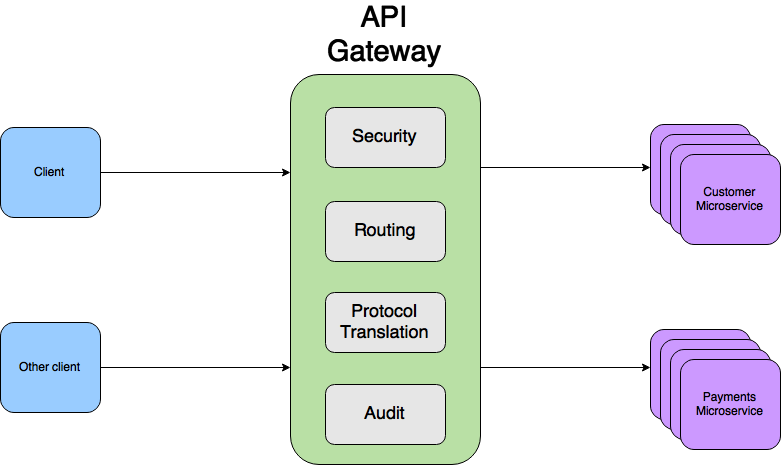
\includegraphics[scale=0.4]{images/AGARC.png}
\end{figure}

\cleardoublepage 
\section{مروری بر منابع}\label{sec:sources}

\subsection{مقدمه}\label{subsec:sources_subject}
در ابتدا ویژگی‌های یک درگاه ارتباط مناسب بررسی شده و سپس برخی از درگاه‌های شناخته‌شده‌ مورد بررسی قرار می‌گیرند که چه میزان از ویژگی‌های یک درگاه ارتباط مناسب را دارا هستند و در نهایت دلایل برتری راه‌حل پیشنهادی به دیگر درگاه‌ها ذکر شده است.


\subsubsection{درگاه ارتباط مناسب}\label{subsec:sources_gateway}
مهم‌ترین ویژگی‌های یک درگاه ارتباط مناسب عبارتند از:

\begin{itemize}
    \item مسیردهی \LTRfootnote{Routing}
    \item قابلیت پیکربندی با روش‌های مختلف
    \item مقیاس‌مندی \LTRfootnote{Scalability}
    \item گسترش‌پذیری \LTRfootnote{Extendability}
    \item توازن بار \LTRfootnote{Load Balancing}
    \item ثبت رخداد‌ها \LTRfootnote{Logging events}
    \item رصد وضعیت سامانه \LTRfootnote{Monitoring}
\end{itemize}

\subsubsection{مسیر‌دهی}
اساسی‌ترین نیاز یک درگاه ارتباطی، مسیر‌دهی با استفاده از مولفه‌های مختلف درخواست از جمله نوع پروتکل، مسیر درخواست، سرتیتر‌های درخواست و... است. تنوع پشتیبانی از مولفه‌های مختلف در مسیر‌دهی باعث می‌شود که درخواست‌ها دقیق‌تر به خدمت مورد‌نظر برسند.

\subsubsection{قابلیت پیگربندی با روش‌‌های مختلف}
با توجه به محیط‌های مختلف برای بارگذاری نرم‌افزارها و تغییر پی‌در‌پی نیازها، درگاه ارتباط باید اطلاعات مورد‌نیاز برای مسیر‌دهی به درخواست‌ها را از روش‌های مختلف کشف و دریافت کند. در این‌صورت در صورت اضافه و یا حذف کردن یک خدمت، نیازی به تغییر در پیکربندی نبوده و درگاه پیکربندی خود را با تغییرات جدید به روز می‌کند.

\subsubsection{مقیاس‌مندی}
با بالا رفتن تعداد درخواست‌ها ممکن است که درگاه ارتباط تبدیل به تک نقطه‌ی شکست
\LTRfootnote{Single Point of Failure}
شود. با قابلیت مقیاس‌مندی این امکان وجود دارد که به صورت هم‌زمان چند درگاه ارتباط مختلف را اجرا کرد و هر‌کدام از این درگاه‌ها به صورت مستقل به درخواست‌ها پاسخ دهند.

\subsubsection{گسترش‌پذیری}
درگاه‌های ارتباط، معمولا به صورت پیش‌فرض طیف نیازهای عمومی تمام سامانه‌ها را پوشش می‌دهند. یکی از قابلیت‌های مناسب برای درگاه ارتباط، امکان گسترش‌پذیری و اضافه کردن نیاز مختص به یک سامانه به درگاه ارتباط است.

\subsubsection{توزان بار}
برای جلوگیری از ایجاد تک نقطه‌ی شکست در معماری میکروسرویس، چند نسخه از یک خدمت اجرا می‌شود. درگاه ارتباط باید بتواند با روش‌های مختلف، بار ورودی به سامانه را بین این نسخه‌ها تقسیم کند.

\subsubsection{ثبت رخداد‌ها و رصد وضعیت سامانه}
در معماری میکروسرویس یک سامانه از اجزای مستقل و مختلفی تشکیل شده است که هر‌کدام وظیفه‌ی مشخصی دارند. یکی از چالش‌های موجود در این معماری رصد کردن خدمت‌های مختلف است. با توجه به اینکه درگاه ارتباط با تمام خدمت‌های یک سامانه در ارتباط است می‌تواند وضعیت تمام خدمت‌ها را در قالب‌های مختلف گزارش کند.


\subsection{مروری بر ادبیات موضوع}\label{subsec:sources_literature}
در این بخش دو درگاه ارتباط محبوب و پرکاربرد Traefik و Kong مورد ارزیابی واقع می‌شوند و مزایا و معایب هر یک مشخص می‌شود.

\subsubsection{درگاه ارتباط Traefik}
درگاه ارتباط Traefik یکی از محبوب‌ترین درگاه‌های ارتباط متن‌باز است که اکثر ویژگی‌های یک درگاه ارتباط مناسب را دارا است. این درگاه ارتباط، با زبان برنامه‌نویسی Golang توسعه داده شده است که این امر باعث بهینگی و عملکرد مناسب آن شده است.

مهم‌ترین ویژگی \lr{Traefik}، سازگاری آن با محیط‌های مختلف بارگذاری نرم‌افزار است. این درگاه ارتباط، به صورت خودکار پیکربندی تمام خدمات را از محیط نرم‌افزار استخراج می‌کند که این امر باعث سادگی در استفاده از آن می‌شود.

بزرگ‌ترین مشکل Traefik عدم گسترش‌پذیری آن است. به صورتی که در صورت نیاز به اضافه کردن یک بخش اختصاصی به آن، راهی به غیر از تغییر در متن وجود ندارد.

\subsubsection{درگاه ارتباط Kong}
Kong درگاه ارتباطی است که بر روی Nginx استوار شده است و در دو نسخه‌ی متن‌باز و تجاری قابل استفاده است. این درگاه ارتباط با استفاده از Nginx به عنوان هسته‌ی خود، قابلیت اتکای بالایی دارد و از تمام مزایای آن استفاده می‌کند.

یکی از مهم‌ترین ویژگی‌های \lr{Kong}، رابط کاربری و پنل مدیریت آن است، که تغییرات در هنگام اجرا را میسر می‌سازد. پنل مدیریت Kong از ویژگی‌های نسخه‌ی
تجاری آن است.

این درگاه ارتباط،‌ با زبان برنامه‌نویسی Lua توسعه داده شده است که با توجه به محبوبیت کم‌تر این زبان، باعث شده‌ است جامعه‌ی برنامه‌نویسی کم‌تر به سراغ توسعه‌ی آن برود. از طرفی گسترش‌پذیری \lr{Kong}، بدون تغییر در متن آن، امری ممکن اما دشوار است.

\subsection{نتیجه‌گیری}\label{subsec:sources_results}
با توجه به بررسی‌های انجام شده،‌ خلا یک درگاه ارتباط با قابلیت گسترش‌پذیری بالا حس می‌شود. معماری این درگاه باید به صورتی باشد که بتوان بدون نیاز به ایجاد تغییر در متن، منطق خاص مورد استفاده در یک سامانه را به آن اضافه کرد.

هم‌چنین با توجه به تنوع در محیط‌های بارگذاری سامانه‌های با معماری میکروسرویس، درگاه ارتباط باید بتواند با اجزاهای محیطی مختلف ارتباط برقرار کرده و تنظیمات مربوط به خدمت‌های مختلف را از این محیط‌ها دریافت کند. نمونه‌هایی از محیط‌های مختلف عبارتند از سکوی
\LTRfootnote{Platform}
\lr{Docker}، \lr{Kubernetes} و... .

درگاه ارتباط پیاده‌سازی شده با تمرکز بر گسترش‌پذیری و قابلیت پیکربندی به عنوان شاخص‌های اصلی نسبت به سایر درگاه‌های موجود پیاده‌سازی شده است. جزئیات مربوط به نحوه‌ی پیاده‌سازی این ویژگی‌ها در فصل
\ref{sec:implementation}
آمده است.

مقایسه‌ی درگاه‌های ارتباط مختلف، در جدول
\ref{tab:gateways}
قابل مشاهده است.


\begin{table}[H]
    \centering
    \caption{مقایسه‌ی درگاه‌های ارتباط مختلف}\label{tab:gateways}
    \begin{tabular}{|c|c|c|c|}
        \hline
         & Traefik & Kong & درگاه ارتباط پیشنهادی\\
        \hline
        مسیردهی & بالا & بالا & بالا\\
        \hline
        قابلیت پیکر‌بندی با روش‌های مختلف & بالا & متوسط & بالا\\
        \hline
        مقیاس‌مندی & بالا & بالا & بالا\\
        \hline
        گسترش‌پذیری & پایین & متوسط & بالا\\
        \hline
        توازن بار & بالا & بالا & متوسط\\
        \hline
        ثبت رخداد‌ها & بالا & بالا & متوسط\\
        \hline
        رصد وضعیت سامانه & بالا & متوسط & بالا\\
        \hline
        سادگی استفاده & بالا & متوسط & بالا\\
        \hline
    \end{tabular}
\end{table}

\cleardoublepage 
\section{روش پیاده‌سازی}\label{sec:implementation}

\subsection{مقدمه}\label{subsec:impl_intro}
برای پیاده‌سازی یک سامانه، می‌توان دو رویکرد داشت. می‌توان از سامانه‌های از پیش موجود استفاده کرد و با حاصل کردن تغییرات لازم به مقصود رسید. و یا می‌توان با پیاده‌سازی سامانه از ابتدا، نیاز‌های را حل کرد.

از طرفی با توجه به ویژگی‌های ذکرشده در فصل
\ref{sec:sources}
، راه حل انتخابی برای پیاده‌سازی یک درگاه ارتباط با رابط‌های برنامه‌نویسی باید معیار‌های زیر را مدنظر خود قرار داده باشد:

\begin{itemize}
    \item سرعت بالا
    \item کارایی بالا
    \item بهینه‌بودن راه‌حل
    \item گسترش‌پذیری
    \item تغییر‌پذیری
    \item سادگی و قابل فهم بودن
\end{itemize}

\subsection{انتخاب روش و فناوری}\label{subsec:impl_choose}
استفاده‌ از فناوری‌های موجود، مانند \lr{Nginx}، \lr{HAProxy} و ... و ایجاد تغییرات در آن‌ها جهت بر طرف کردن نیاز‌های مطرح شده در فصل
\ref{sec:sources}
، می‌تواند یکی از راه‌حل ‌های حل مسئله باشد. ولی با توجه به پایه‌ی پیاده‌سازی این محصولات بر اساس نیاز‌های گذشته، و همچنین عدم سازگاری این محصولات با محیط‌های ابری، جهت استفاده به عنوان درگاه ارتباط با رابط‌های برنامه‌نویسی، مشکلات زیادی برای حل مسئله وجود خواهد آمد. برخی از این مشکلات عبارتند از:

\begin{itemize}
    \item اجبار به استفاده از راه‌حل‌های موقتی برای سازگاری این محصولات با فضای موجود
    \item پیچیدگی بیش از حد به دلیل وجود ویژگی‌های مرتبط با حوزه‌های دیگر
    \item احتمال عدم سازگاری تغییرات مورد نظر با ویژگی‌های اصلی محصول
    \item و \ldots
\end{itemize}

از این رو پیاده‌سازی یک درگاه، از ابتدا و با توجه به نیاز‌های جدید،‌ راه حل منطقی تری به نظر می‌رسد.

با توجه به نیاز سامانه‌ به دسترسی‌های سطح پایین، جهت ارتباط با لایه‌ی هفتم شبکه، و همچنین نیاز به سرعت بالا برای کنترل بار، زبان‌های برنامه‌نویسی محدودی مناسب پیاده‌سازی این محصول خوا‌هند بود. برخی از این گزینه‌ها عبارتند از:

\begin{itemize}
    \item زبان برنامه‌نویسی کامپایلری C/C++
    \item زبان برنامه‌نویسی کامپایلری Golang
    \item زبان برنامه‌نویسی مفسری Lua
    \item زبان برنامه‌نویسی Javascript (بستر \lr{Node.js})
\end{itemize}

معمولا زبان‌های برنامه‌نویسی سطح پایین‌تر، سرعت بالاتری نیز دارند. از این رو زبان‌های C و C++ از بالاترین سرعت برخوردار هستند. با این وجود، کاری‌هایی مانند مدیریت حافظه، مدیریت پردازه‌های هم‌روند و ... به عهده‌ی برنامه‌نویس است. این امر باعث پیچیدگی توسعه خواهد بود. از این رو، زبان برنامه‌نویسی Golang، که یک زبان برنامه‌نوسی سطح‌ پایین محسوب می‌شود، به علت مدیریت حافظه خودکار و استفاده‌ی ساده از پردازه‌ها
\LTRfootnote{Process}
و ریسمان‌ها
\LTRfootnote{Thread}
برای اجرای فرآیند‌های هم‌روند، می‌تواند گزینه‌ی مناسبی جهت پیاده‌سازی باشد.

از زبان‌های مفسری نیز می‌توان برای توسعه‌ی نرم‌افزار‌هایی که در زمان اجرا نیاز به تغییر در خود دارند، استفاده کرد. ولی نقطه‌ی تاریک استفاده ‌از زبان‌های برنامه‌نویسی مفسری، احتمال بالای رخداد خطا‌های زمان اجرا خواهد بود. این ویژگی باعث از دست رفتن ثبات سامانه می‌شود.

نحوه‌ی انجام فرآیند‌های هم‌روند نیز در انتخاب فناوری پیاده‌سازی این بخش از سامانه بسیار تاثیرگذار است. زیرا با توجه به نیاز به توان عملیاتی بالا، فناوری‌های تک رشته‌ای و یا تک‌ پردازه‌ای باعث کاهش توان عملیاتی سامانه خواهند شد.

جدول
\ref{tab:choice}
شامل مقایسه‌ی زبان‌های برنامه‌نویسی ذکر شده با توجه‌ به معیار‌های ذکر شده است.

\begin{table}[H]
    \centering
    \caption{مقایسه‌ی زبان‌های برنامه‌نویسی جهت پیاده‌سازی درگاه ارتباط با رابط‌های برنامه‌نویسی}\label{tab:choice}
    \begin{tabular}{|c|c|c|c|c|c|c|}
        \hline
        زبان برنامه‌نویسی & سرعت & سادگی & بهینگی & توان عملیاتی & مدیریت حافظه & مدیریت فرآیند‌های هم‌روند\\
        \hline
        C/C++ & بسیار بالا & پایین & بسیار بالا & بسیار بالا & خیر & بسیار سخت\\
        \hline
        Golang & بالا & متوسط & بالا & بالا & بله & آسان\\
        \hline
        Lua & بالا & متوسط & بالا & متوسط & بله & سخت\\
        \hline
        Javascript & متوسط & بالا & پایین & متوسط & بله & سخت\\
        \hline
    \end{tabular}

\end{table}


با توجه به جدول
\ref{tab:choice}
، روش انتخابی برای حل مسئله،‌ پیاده‌سازی سامانه از ابتدا و با استفاده از زبان برنامه‌نویسی Golang است. زیرا با اینکه سرعت کمتری نسبت به زبان برنامه‌نویسی C یا C++ دارد، ولی با توجه به عدم نیاز به مدیریت حافظه، مدیریت آسان‌تر فرآیند‌های هم‌روند و همچنین سادگی و بهینگی قابل قبول،‌ می‌توان از اختلاف سرعت این دو زبان برنامه‌نویسی چشم پوشی کرد.

\subsection{پیاده‌سازی}\label{subsec:impl_impl}

\subsubsection{ساختار}
ساختار برنامه‌ باید به شکلی تعیین شود که برنامه‌نویس را در روند توسعه برنامه محدود نکند. علاوه بر این، یک ساختار خوب می‌تواند زمینه را جهت معماری گسترش‌پذیر و منعطف فراهم کند.

یکی از ساختار‌های مناسب، در محیط توسعه‌ی Golang ، ساختار بسته مبنا است. این ساختار توسط بسیاری از محصولات صنعتی و آکادمیک استفاده شده است. همچنین برخی از ابزار‌های از پیش‌آماده در محیط توسعه‌ی این زبان، از سازگاری کامل با این ساختار برخوردار هستند.

\subsubsection{ساختار بسته‌مبنا}
این ساختار، شامل سه پوشه‌ی اصلی \lr{cmd}، \lr{internal} و \lr{pkg} است. پوشه‌های config و logging از جمله پوشه‌های دیگر این ساختار هستند که استفاده از آن‌ها توصیه شده است.

پوشه‌ی cmd حاوی برنامه‌ی اصلی و قابل اجرا است. این پوشه معمولا دارای برنامه‌های کوتاه و با منطق ساده هستند.

پوشه‌ی pkg حاوی بسته‌های مستقل و قابل استفاده توسط سایر برنامه هاست. بسته‌های موجود در این پوشه به تنهایی قابل استفاده اند و وابستگی آن‌ها به دیگر بسته ها بسیار کم است.

پوشه‌ی internal دارای بسته‌هایی است که از بسته‌های موجود در pkg استفاده کرده و منطق اصلی برنامه را پیاده‌سازی می‌کند. در این پوشه، رابط‌های ورودی و خروجی برنامه تعیین می‌شود.

بسته‌ی logging شامل برنامه‌های مربوط به ثبت اتفاقات سامانه است.

بسته‌ی config نیز دربردارنده‌ی برنامه‌های مربوط به پیکربندی و تنظیمات اجرای برنامه است. نحوه‌ی بارگذاری پیکربندی‌ها و همچنین استفاده از تنظیمات در قسمت‌های مختلف برنامه در این قسمت پیاده‌سازی می‌شود.

نمونه‌ی یک ساختار بسته‌مبنا در شکل
\ref{package_oriented}
قابل مشاهده است.

\begin{figure}[H]
    \centering
    \caption{نمونه‌ی یک ساختار بسته مبنا}
    \label{package_oriented}
    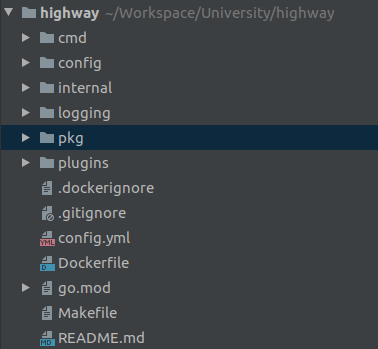
\includegraphics[scale=0.4]{images/PackageOriented.png}
\end{figure}

\cleardoublepage

\subsection{مفاهیم}\label{subsec:impl_concepts}
برای پیاده‌سازی یک درگاه ارتباط با رابط‌های برنامه‌نویسی، مفاهیم زیر پیشنهاد شده است:

\begin{itemize}
    \item بطن \LTRfootnote{Backend}
    \item خدمت \LTRfootnote{Service}
    \item متعادل‌کننده‌ی بار \LTRfootnote{Load Balancer}
    \item ضابطه \LTRfootnote{Rule}
    \item میان‌افزار \LTRfootnote{Middleware}
    \item مسیریاب \LTRfootnote{Router}
    \item تامین کننده‌ی خدمت \LTRfootnote{Service Provider}
\end{itemize}

در ادامه به توضیح هر یک از مفاهیم ذکر‌ شده پرداخته‌ می‌شود.

\subsubsection{بطن}
یک بطن، کوچک‌ترین واحد در این سامانه است. هر بطن، یک داده ساختار شامل نام، آدرس، وزن و وضعیت است. این چهار ویژگی نشان‌دهنده‌ی یک نمونه از رابط‌های برنامه‌نویسی قابل استفاده توسط برنامه است. داده‌ساختار زیر، نشان‌دهنده‌ی بطن است.

\begin{latin}
    \begin{lstlisting}
                                    type Backend struct {
                                        Name string
                                        Addr string
                                        Weight int8
                                        Status int
                                    }
    \end{lstlisting}
\end{latin}


\subsubsection{خدمت}
یک خدمت دارای یک نام، چند بطن و یک متعادل‌کننده‌ی توزیع بار است. معمولا بطن‌های یک خدمت کاملا مشابه یکدیگر عمل می‌کنند. با توجه به قسمت
\ref{subsubsec:impl_loadbalancer}
، خدمت با استفاده از متعادل‌کننده‌ی بار درخواست‌های را بین بطن‌های خود توزیع می‌کند.

قطعه کد زیر نشان‌دهنده‌ی داده‌ساختار یک خدمت است.

\begin{latin}
    \begin{lstlisting}
                                    type Service struct {
                                        Name     string
                                        Backends []Backend
                                        LB       LoadBalancer
                                    }
    \end{lstlisting}
\end{latin}

\subsubsection{متعادل‌کننده‌ی بار}\label{subsubsec:impl_loadbalancer}
این موجودیت در برنامه از نوع یک واسط
\LTRfootnote{Interface}
است. این واسط بدون در نظر گرفتن منطق پیاده‌سازی توزیع بار، رفتار‌های مورد نیاز برای این عمل را مشخص می‌کند.

این واسط به طور مستقیم قابل استفاده نیست. بلکه نسخه‌های پیاده‌سازی شده‌ی این واسط را می‌توان به طور مستقیم استفاده کرد. برای مثال، الگوریتم توزیع تصادفی جهت توزیع بار در این برنامه پیاده‌سازی شده است. برنامه‌ی زیر نشان‌دهنده‌ی واسط متعادل‌کننده‌ی بار و شکل
\ref{service_package}
حاوی نمودار پیاده‌سازی نمونه‌ها از واسط هستند.


\begin{latin}
    \begin{lstlisting}
                                    type LoadBalancer interface {
                                        Balance([]Backend) Backend
                                    }
    \end{lstlisting}
\end{latin}


\begin{figure}[H]
    \centering
    \caption{نمودار UML بسته‌ی Service}
    \label{service_package}
    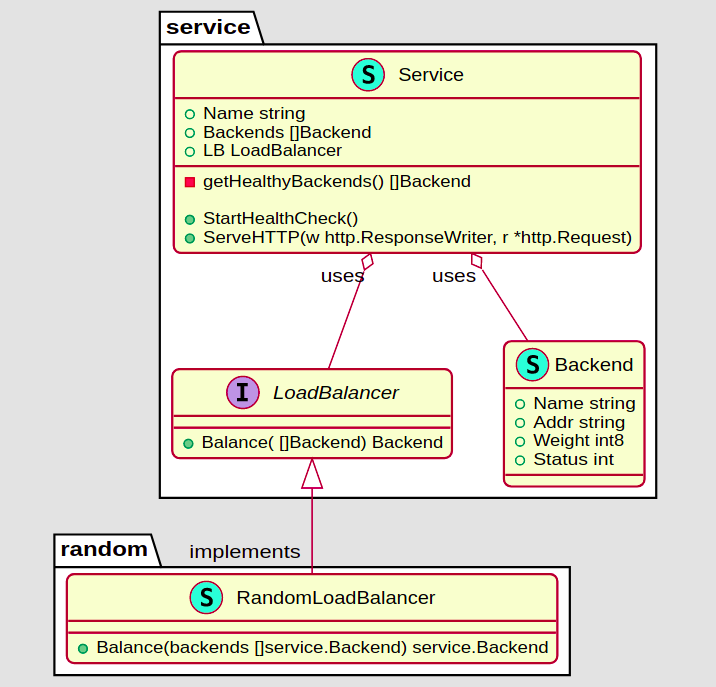
\includegraphics[scale=0.2]{images/Loadbalance.png}
\end{figure}

متعادل‌کننده‌های بار می‌توانند از وزن بطن‌های یک سرویس، برای توزیع وزن‌دار بار استفاده‌ کنند.


\subsubsection{تامین کننده‌ی خدمت‌ها}
تامین‌کننده‌ وظیفه تامین پیکربندی‌ خدمت‌های مختلف را دارد. با توجه به تنوع در محیط‌های بارگذاری سامانه‌های با معماری میکروسرویس، درگاه ارتباط باید بتواند با اجزاهای محیطی مختلف ارتباط برقرار کرده و تنظیمات مربوط به خدمت‌های مختلف را از این محیط‌ها دریافت کند. قطعه کد زیر نشان‌دهنده‌ی واسط مربوط به تامین کننده‌ی خدمت است.

\begin{latin}
    \begin{lstlisting}
                                    type ServiceProvider interface {
                                        Provide() ([]service.Service, error)
                                        Watch(messageChan chan<- Message) error
                                    }
    \end{lstlisting}
\end{latin}

تامین‌کننده به صورت یک واسط تعریف شده است و نسخه‌های پیاده‌سازی شده‌ی مختلف ‌آن‌ها، پیکربندی‌های مختلف را از محیط‌های متفاوت مانند \lr{Docker}، ‌\lr{Kubernetes} و ... جمع‌آوری می‌کنند.

شکل
\ref{provider}
نشان‌دهنده‌ی نمودار UML و نسخه‌های پیاده‌سازی شده از تامین‌کننده‌ی خدمت‌هاست.

\begin{figure}[H]
    \centering
    \caption{نمودار UML بسته‌ی Provider}
    \label{provider}
    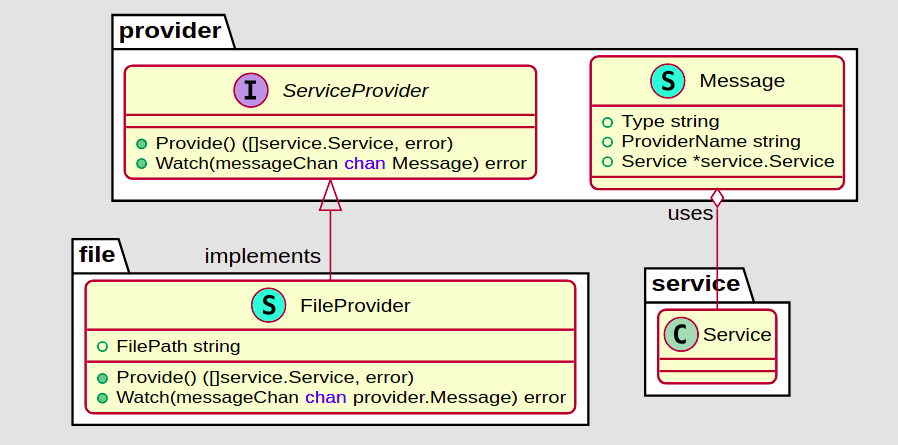
\includegraphics[scale=0.2]{images/Provider.png}
\end{figure}

\subsubsection{ضابطه}
ضابطه‌ها داده‌ساختار‌هایی هستند که می‌توان از طریق آن‌ها به خدمات دسترسی پیدا کرد. در قالب این گزارش، ضابطه‌ها تنها برای پروتکل‌های HTTP و HTTPS طراحی شده‌اند. با توجه به ویژگی‌های این پروتکل‌ها، ضابطه‌های مختلفی می‌توان تعریف کرد. برخی از این ویژگی‌ها عبارتند از:

\begin{itemize}
    \item نوع پروتکل (\lr{HTTP} یا \lr{HTTPS})
    \item مسیر درخواست \LTRfootnote{Path}
    \item آدرس میزبان درخواست \LTRfootnote{Host}
    \item نوع درخواست \LTRfootnote{Request Method}
    \item سرتیتر‌های درخواست \LTRfootnote{Headers}
    \item مولفه‌های پرس‌و‌جوی درخواست \LTRfootnote{Query Params}
    \item میان‌افزار‌ها
\end{itemize}

کاربرد و نحوه‌ی استفاده از میان‌افزار ها در قسمت
\ref{subsubsec:impl_middleware}
بررسی خواهد شد.


قطعه کد زیر، نمایان‌گر داده‌ساختار یک ضابطه است.

\begin{latin}
    \begin{lstlisting}
                                    type Rule struct {
                                        Service     *service.Service
                                        Schema      string
                                        PathPrefix  string
                                        Hosts       []string
                                        Methods     []string
                                        Headers     map[string]string
                                        Queries     map[string]string
                                        Middlewares []middlewares.Middleware
                                        handler     http.HandlerFunc
                                    }
    \end{lstlisting}
\end{latin}

\subsubsection{میان‌افزار}\label{subsubsec:impl_middleware}
گاهی نیاز است قبل از رسیدن درخواست به خدمت، تغییراتی در درخواست ایجاد شود. و یا برخی از سیاست‌های کنترلی مانند احراز هویت و تایید دسترسی قبل از رسیدن درخواست به خدمت بررسی شود.

در برخی از مواقع نیز این نیاز مطرح است که از نتایج درخواست‌ها مطلع شد و از آن‌ها برای تولید گزارشات و تهیه‌ی داده‌های آماری استفاده کرد.

میان‌افزار‌ها این نیاز‌ها را برطرف خواهند کرد. میان‌افزار‌ها نیز به صورت یک واسط تعریف شده‌اند و نسخه‌های پیاده‌سازی شده‌ی مختلف ‌آن‌ها نیاز‌های مختلف را رفع خواهند کرد. برنامه‌ی زیر نشان‌دهنده‌ی شمای این واسط است.

\begin{latin}
    \begin{lstlisting}
                        type Middleware interface {
                            Process(handler http.HandlerFunc) http.HandlerFunc
                        }
    \end{lstlisting}
\end{latin}

در سامانه‌ی پیاده‌سازی شده، میان‌افزار ها دو قسم اند. برخی از آن‌ها،‌که معمولا جز میان‌افزار‌های پرطرفدار در صنعت هستند، به صورت پیشفرض پیاده‌سازی شده‌اند.
میان‌افزار‌های از پیش آماده در این سامانه عبارتند از:

\begin{itemize}
    \item میان‌افزار CORS
    \item میان‌افزار محدود‌کننده‌ی نرخ درخواست \LTRfootnote{Rate limiter}
    \item میان‌افزار رصد سامانه
\end{itemize}

محدود‌کننده‌ی نرخ درخواست با استفاده از الگوریتم \lr{Token Bucket}
\cite{tokenbucket}
باعث می‌شود بتوان نرخ ارسال درخواست‌های کاربران را تحت کنترل قرار داد.

میان‌افزار CORS
\cite{cors}
نیز با استفاده از استاندارد‌های تعیین‌شده برای درخواست‌های با مبدا و مقصد مختلف، دسترس‌پذیری این سامانه‌ را از منابع مختلف تعیین می‌کند.

میان‌افزار رصد سامانه نیز، طبق استاندارد‌های نرم‌افزار \lr{Prometheus}،
\cite{prometheus}
امکان بررسی و تحلیل اطلاعات را فراهم می‌کند.

گروهی دیگر از میان‌افزار‌ها نیز توسط کاربران سامانه تعریف و پیاده‌سازی شده و به داخل سامانه تزریق می‌شوند. این ویژگی باعث می‌شود استفاده کنندگان از این سامانه، هیچ‌گونه وابستگی به توسعه‌دهندگان اصلی برنامه نداشته باشند و میان‌افزار‌های مربوط‌ به نیازمندی‌های خاص خود را پیاده‌سازی کرده و در سامانه تزریق کنند.

شکل
\ref{middlewares_package}
نشان‌دهنده‌ی نحوه‌ی پیاده‌سازی میان‌افزار‌ها با استفاده از واسط تعیین‌شده است.

\begin{figure}[H]
    \centering
    \caption{نمودار UML بسته‌ی Middleware}
    \label{middlewares_package}
    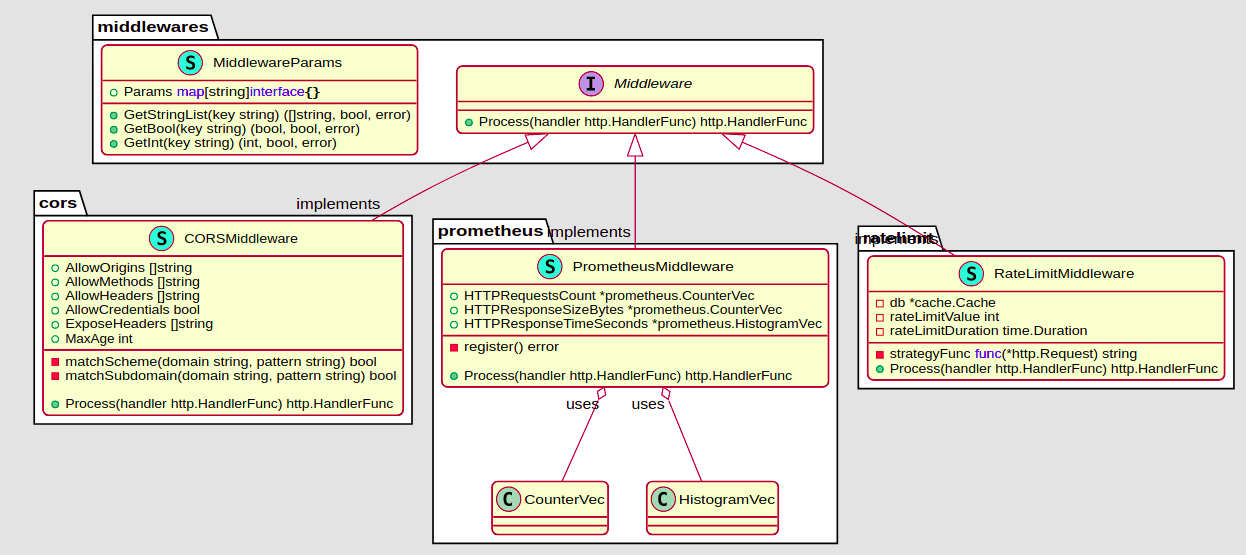
\includegraphics[scale=0.2]{images/Middleware.png}
\end{figure}

\subsubsection{مسیریاب}\label{subsec:impl_router}
یک درگاه ارتباط با رابط‌های برنامه‌نویسی را می‌توان یک مسیریاب لایه‌ی هفتم شبکه در نظر گرفت. بدین صورت که درخواست‌های ارسالی از سمت کاربران را به پاسخ‌دهنده‌های مربوط به آن‌ درخواست‌ها هدایت می‌کند.

یک مسیریاب به طور واسط تعریف شده‌ است و رفتار‌های مورد نیاز آن، بدون توجه به منطق پیاده‌سازی آن مشخص شده است. برنامه‌ی زیر تعریف یک واسط مسیریاب را نشان می‌دهد.

\cleardoublepage

\begin{latin}
    \begin{lstlisting}
                            type Router interface {
                                AddRule(rule rules.Rule) error
                                ServeHTTP(w http.ResponseWriter, req *http.Request)
                            }
    \end{lstlisting}
\end{latin}

مسیریاب‌ها با استفاده از ضابطه‌های تعریف‌شده، هر درخواست را به خدمت مورد نظر هدایت می‌کنند.

شکل
\ref{router_package}
نشان‌دهنده‌ی نحوه‌ی پیاده‌سازی یک مسیریاب با استفاده ‌از واسط تعیین شده است.

\begin{figure}[H]
    \centering
    \caption{نمودار UML بسته‌ی Router}
    \label{router_package}
    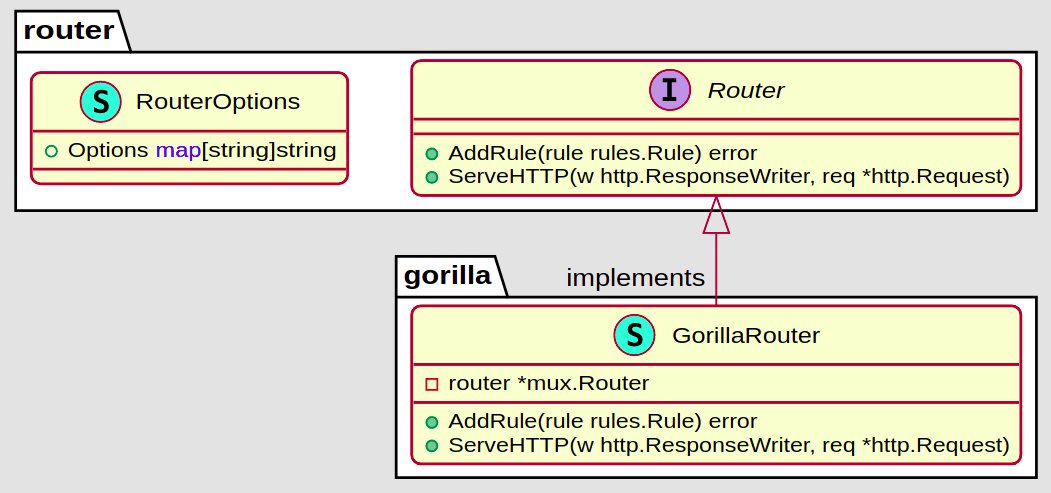
\includegraphics[scale=0.2]{images/Router.png}
\end{figure}

به طور کلی، شکل
\ref{flow}
نشان‌دهنده‌ی روند طی‌شده برای درخواست کاربران را به طور خلاصه شرح می‌دهد.

\begin{figure}[H]
    \centering
    \caption{روند طی‌شده برای هر درخواست}
    \label{flow}
    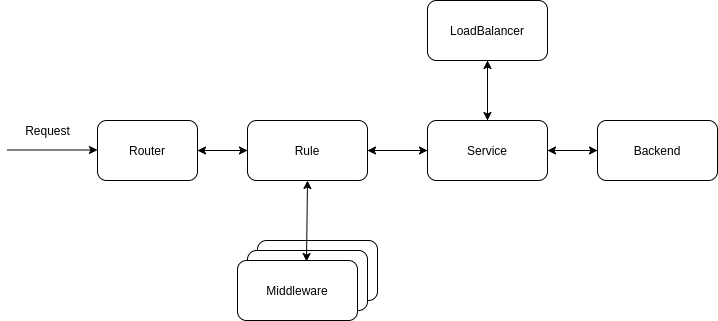
\includegraphics[scale=0.4]{images/Flow.png}
\end{figure}

\subsection{ویژگی‌های سامانه}\label{subsec:impl_features}
معماری ذکر‌شده در بخش
\ref{subsec:impl_concepts}
، ویژگی‌های زیر را داراست:

\begin{itemize}
    \item کمترین وابستگی ممکن
    \item آزمون پذیری بالا
    \item گسترش پذیری بالا
    \item مقیاس‌مندی بالا
\end{itemize}

\subsubsection{وابستگی}
با استفاده درست از واسط‌ها و همچنین طراحی ماژولار، بخش‌های مختلف سامانه کمترین وابستگی به یکدیگر را دارند. این ویژگی باعث می‌شود تغییرات احتمالی در آینده به راحتی هرچه تمام‌تر انجام شود.

\subsubsection{آزمون‌پذیری}
با توجه به وابستگی کم اجزای سامانه به یکدیگر،‌هر یک از اجزا می‌توانند به تنهایی مورد آزمون و ارزیابی قرار گیرند.
هم‌چنین استفاده از واسط‌ها امکان ایستا کردن یک بخش و انجام آزمون واحد
\LTRfootnote{Unit test}
بر روی بخش دیگر را امکان‌پذیر می‌کند.

\subsubsection{گسترش‌پذیری}
با توجه به استفاده به موقع از واسط‌ها، گسترش سامانه،‌ از طریق پیاده‌سازی نسخه‌های جدید از واسط‌ها، بسیار ساده خواهد بود. همچنین امکان تزریق میان‌افزار‌های پیاده‌سازی شده توسط کاربران استفاده کننده، بدون نیاز به کامپایل مجدد نرم‌افزار، خاصیت گسترش پذیری نرم‌افزار را افزایش می‌دهد.

\subsubsection{مقیاس‌مندی}
با توجه به عدم ذخیره‌ی حالت در سامانه، می‌توان تعداد نسخه‌های در حال اجرای سامانه‌ را به طور خطی برای افزایش میزان توان عملیاتی سامانه، زیاد کرد.

\cleardoublepage 
\section{نتایج و تفسیر آن‌ها}\label{sec:results}
پس از پیاده‌سازی معماری شرح‌داده‌شده در فصل
\ref{sec:implementation}
، آزمایش کیفیت و نحوه‌ی عملکرد سامانه ضروری به نظر می‌رسد. در آزمایش‌های انجام‌شده، سامانه‌ی پیاده‌سازی شده با یکی از محبوب‌ترین نمونه‌های صنعتی، به نام \lr{Kong}، مورد مقایسه قرار گرفته شده ‌است. در ادامه، به نحوه‌ی انجام آزمایش پرداخته شده است.


\subsection{محیط آزمایش}\label{subsec:results_env}
با توجه به کاربرد وسیع درگاه‌های ارتباط با رابط‌های برنامه‌نویسی در محیط‌های ابری، انجام این آزمایش در محیط ابری به واقعیت نزدیک‌تر خواهد بود. از این رو تمام آزمایش‌ها در محیط ابری انجام شده‌است. آزمایش‌ها بر روی بستر OKD
\LTRfootnote{Openshift Kubernetes Distribution}
انجام شده‌اند.

برای ایجاد بار بر روی سامانه‌های مورد آزمایش از سکوی Locust استفاده شده است. میزان منابع مصرفی این سکو برای ایجاد بار به شرح زیر است:

\begin{itemize}
    \item میزان حافظه‌ی موقت مصرفی: ۱۱ گیگابایت
    \item تعداد هسته‌های پردازشی: ۲۲
    \item تعداد ایجاد‌کننده‌های بار: ۱۰
\end{itemize}

\subsection{شرح آزمایش‌ها}\label{subsec:results_tests}


\subsubsection{میزان تحمل بار}
برای بررسی میزان تحمل بار، پس از ساخت دو بطن مشابه و بدون سربار بالا، در قالب یک خدمت و استفاده از یک ضابطه‌ی مناسب به انجام آزمایش مبادرت شده است. این فرآیند در هر دو سامانه‌ی مورد ارزیابی انجام شده است.

نتایج حاصل از تولید‌ بار بر هر یک از سامانه‌ها، که در شکل‌های
\ref{highway}
و
\ref{kong}
قابل مشاهده است به شرح زیر است.

\begin{figure}[H]
    \centering
    \label{highway}
    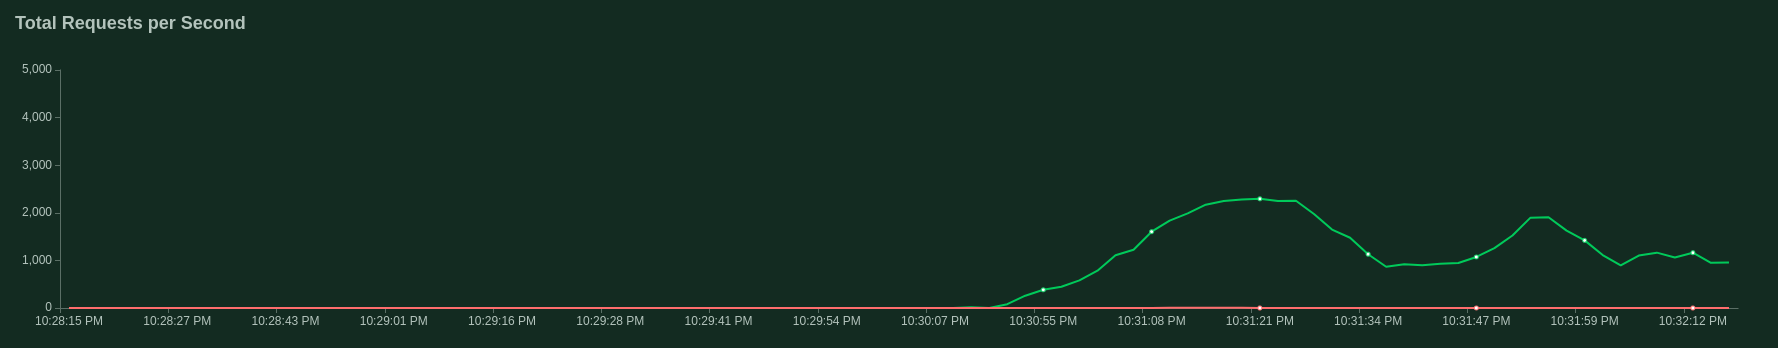
\includegraphics[scale=0.25]{images/HighwayStats.png}
    \caption{نمودار درخواست‌های سامانه‌ی پیاده‌سازی شده}
\end{figure}

\begin{figure}[H]
    \centering
    \label{kong}
    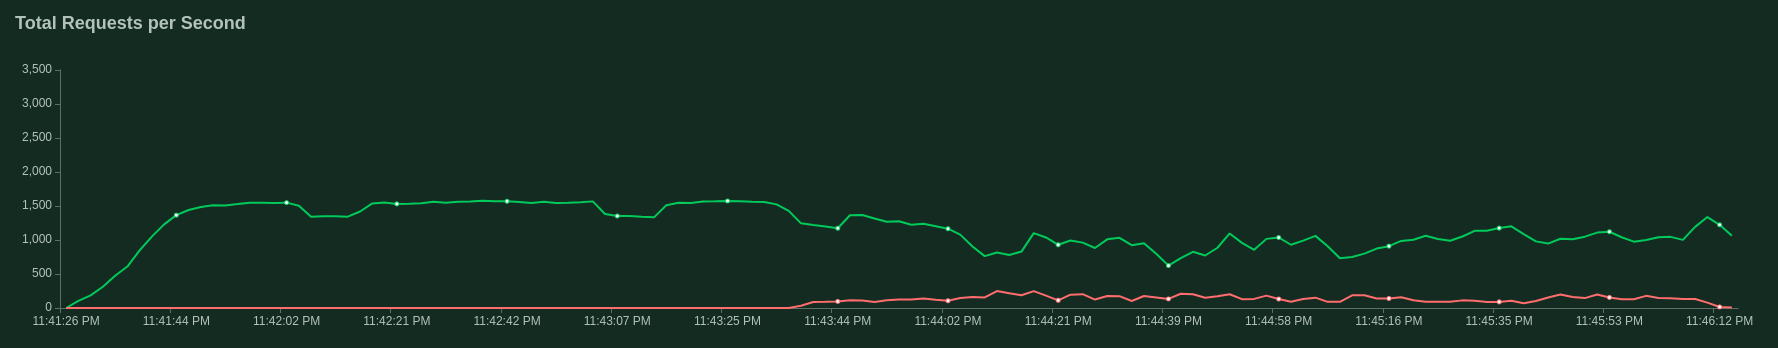
\includegraphics[scale=0.25]{images/KongStats.png}
    \caption{نمودار درخواست‌های Kong}
\end{figure}

\begin{table}[H]
    \centering
    \caption{مقایسه‌ی Kong و سامانه‌ی پیاده‌سازی شده}\label{tab:kongvshighway}
    \begin{tabular}{|c|c|c|c|}
        \hline
        محصول مورد آزمایش & بیشینه مصرف حافظه‌ی موقت & بیشینه مصرف هسته‌های پردازشی & بیشینه میزان تحمل بار\\
        \hline
        سامانه‌ی پیاده‌سازی شده & MB ۲۴۴  & ۲ & rps ۲۳۳۰ \\
        \hline
        Kong & MB ۲۰۴۸ & ۲ & rps ۱۶۴۰ \\
        \hline
    \end{tabular}
\end{table}

با توجه به جدول شماره‌ی
\ref{tab:kongvshighway}
، علی رغم کاهش ٪ ۸۸ ای میزان مصرف حافظه‌ی موقت، بیشینه میزان تحمل بار حدود ٪ ۴۲ افزایش یافته است. علاوه بر این طبق شکل شماره‌ی
\ref{highway}
، میزان درخواست‌های رد شده در سامانه‌ی پیاده‌سازی شده صفر است ولی در سامانه‌ی Kong شاهد رد شدن برخی از درخواست‌ها در اوج بار هستیم.

از این نظر، سامانه‌ی پیاده‌سازی شده بر Kong برتری کامل دارد.

\subsubsection{نحوه‌ی توزیع بار}
با توجه به وجود دو بطن برای سرویس مورد آزمایش، نحوه‌ی عملکرد توزیع‌کننده‌ی بار نیز باید مورد آزمایش قرار گیرد. با فعال کردن میان‌افزار Prometheus بر روی یک ضابطه‌ی جدید و اجرای آزمایش بر روی آن و همچنین تحلیل نتایج حاصل، می‌توان نتایج را در شکل شماره‌ی
\ref{load}
مشاهده کرد.

\begin{figure}[H]
    \centering
    \label{load}
    
\includegraphics[scale=0.23]{images/LoadBalanceStats.png}
    \caption{نحوه‌ی عملکرد توزیع‌کننده‌ی بار}
\end{figure}

با توجه به شکل شماره‌ی
\ref{load}
، از مجموع ۱۸۰۸۷۵ درخواست ارسال شده به سامانه، ۹۰۵۵۲ به بطن اول و ۹۰۳۰۵ به بطن دوم هدایت شده اند. در مجموع ٪ ۵۰/۰۷ درخواست ها به بطن اول و ٪ ۴۹/۹۳ از درخواست‌ها به بطن دوم هدایت شده‌اند. با توجه به وزن یکسان هر دو بطن، نحوه‌ی عملکرد توزیع‌کننده بار، قابل قبول است.


\subsubsection{کنترل نرخ درخواست‌ها}
یکی از میان‌افزار‌های پیاده‌سازی شده، کنترل کننده‌ی نرخ درخواست‌ها است. برای ارزیابی این میان‌افزار و عملکرد درست آن، با ساخت یک ضابطه‌ی جدید و فعال‌سازی این میان‌افزار در آن،‌به اجرای دوباره‌ی آزمایش مبادرت شده است. نحوه‌ی پاسخ به درخواست‌ها توسط سامانه، در شکل
\ref{rate}
قابل مشاهده است.

\begin{figure}[H]
    \centering
    \label{rate}
    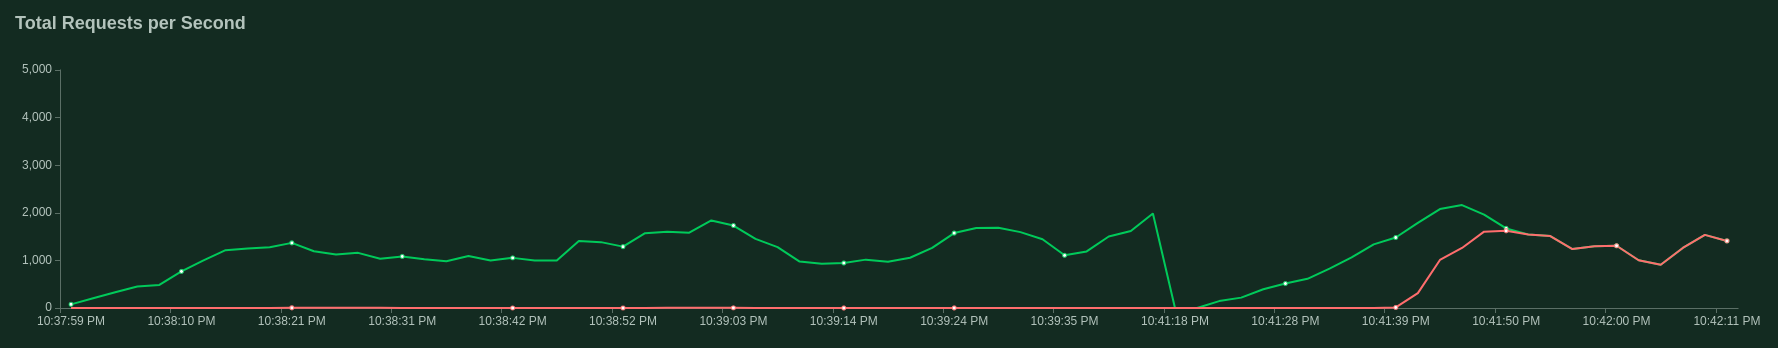
\includegraphics[scale=0.23]{images/RatelimitStats.png}
    \caption{نحوه‌ی رفتار سامانه در حضور کنترل کننده‌ی نرخ درخواست‌ها}
\end{figure}

با توجه به شکل
\ref{rate}
،‌ پس از تمام شدن تعداد درخواست مجاز هر فرستنده در زمان ۱۰:۴۱:۳۹، سامانه شروع به رد کردن درخواست‌های جدید می‌کند. از این رو، میان‌افزار پیاده‌سازی شده به درستی عمل می‌کند.

\subsubsection{رصد و تحلیل سامانه}
برای بررسی عملکرد مطلوب میان‌افزار Prometheus جهت رصد و تحلیل این سامانه، این میان‌افزار در یک ضابطه‌فعال شده و ارزیابی مجددا انجام شده است. در شکل شماره‌ی
\ref{monitoring}
، شاهد نمونه‌ی صفحه‌ی رصد سامانه هستیم. در این صفحه نحوه‌ی عملکرد توزیع‌کننده‌ی بار و همچنین Quantile های مختلف مدت زمان پاسخ‌گویی سامانه محاسبه شده است.

\begin{figure}[H]
    \centering
    \label{monitoring}
    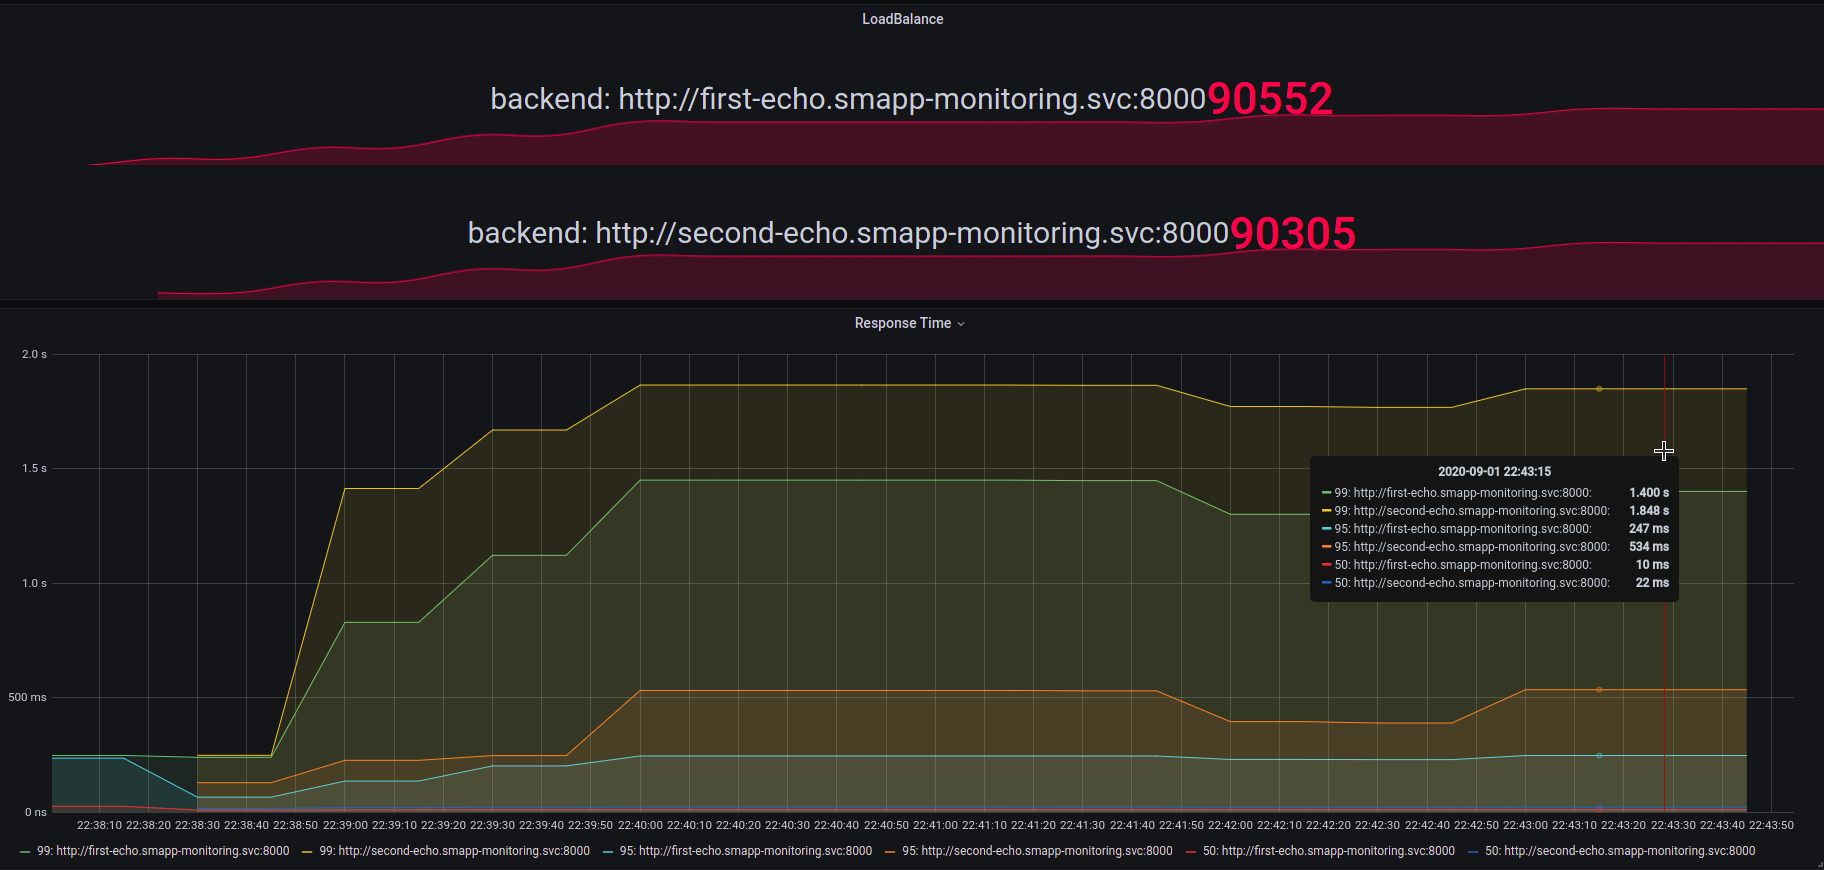
\includegraphics[scale=0.23]{images/Stats.png}
    \caption{نمونه‌ی صفحه‌ی رصد سامانه}
\end{figure}


\cleardoublepage 
\section{جمع‌بندی و پیشنهاد‌ها}\label{sec:recom}

\subsection{مقدمه}\label{subsec:recom_intro}
متن مقدمه

\subsection{محتوا}\label{subsec:recom_mohtava}
متن مقدمه

\subsubsection{جمع‌بندی}
متن‌ها

\subsubsection{نوآوری}
متن‌ها

\subsubsection{پیشنهاد‌ها}
متن‌ها



\cleardoublepage 

\section*{واژه‌نامه فارسی به انگلیسی}\label{sec:gloss}
\addcontentsline{toc}{section}{\numberline{} واژه‌نامه فارسی به انگلیسی}
\thispagestyle{empty}

\englishgloss{Microservice}{میکرو سرویس}
\englishgloss{Monolithic}{یک‌پارچه}
\englishgloss{Centralized}{متمرکز}
\englishgloss{System}{سامانه}
\englishgloss{Interface}{رابط}
\englishgloss{API (Application Programming Interface)}{رابط‌ برنامه نویسی}
\englishgloss{API Gateway}{درگاه ارتباط با رابط‌های برنامه‌نویسی}
\englishgloss{Routing}{مسیردهی}
\englishgloss{Router}{مسیریاب}
\englishgloss{Scalability}{مقیاس‌مندی}
\englishgloss{Extendability}{گسترش پذیری}
\englishgloss{Load Balancing}{توازن بار}
\englishgloss{Monitoring}{رصد}
\englishgloss{Single Point of Failure}{تک نقطه‌ی شکست}
\englishgloss{Platform}{سکو}
\englishgloss{Process}{پردازه}
\englishgloss{Thread}{ریسمان}
\englishgloss{Package Oriented}{بسته‌مبنا}
\englishgloss{Backend}{بطن}
\englishgloss{Service}{خدمت}
\englishgloss{Load Balancer}{متعادل‌کننده‌ی بار}
\englishgloss{Rule}{ضابطه}
\englishgloss{Middleware}{میان‌افزار}
\englishgloss{Service Provider}{تامین‌کننده‌ی خدمت}
\englishgloss{Unit Test}{آزمون واحد}
\englishgloss{Authentication}{احراز هویت}
\englishgloss{Authorization}{کنترل دسترسی}

\cleardoublepage


\bibliographystyle{IEEEtran}
\setLTRbibitems
\addcontentsline{toc}{section}{\numberline{} مراجع}
\bibliography{/home/miladibra/Workspace/University/BachelorThesis/thesis/references/references.bib}

\newpage
\thispagestyle{empty}
\begin{latin}
    \subsection*{Abstract}
    Due to the growth of online businesses and the need for stability and high efficiency for providing services for customers, new architectures should be used for software development. The main characteristics of these architectures are scalability and being fault-tolerant.

    Microservice, among these architectures, is one of the most popular ones. The focus of this architecture is on scalability, extendability and independence of different services from each other. The way this architecture achieves the mentioned features is through separating different functionalities into different services and deploying them in isolated environments.

    Similar to any architecture, the proper implementation of microservice architecture has several challenges. Due to the decentralized nature of the systems in this architecture, connecting users to the services, will not be as simple as in the past because the user needs to gather information from different parts of the system. Therefore, changing the way users communicate with the system and upgrading user applications will be expensive.

    API Gateway pattern is designed to solve this challenge. In this pattern, users still send their requests to only one median system. The task of this median system is to receive requests and redirect them to associated services.

    In spite of the existence of various open source and enterprise API Gateways, most of them lack extendability and configurability. The main purpose of this project is to implement an API Gateway that is extendable and configurable.

    \noindent {\bf Keywords:} API Gateway, Microservice architecture, Decentralized systems, Extendable systems.
\end{latin}
\cleardoublepage
\newpage
\thispagestyle{empty}
\begin{latin}
    \title{
        \center
        
\includegraphics[width=5cm, height=5cm]{images/IUST_logo_color.png} \\ [10pt]
        Computer Engineering Department \\ [40pt]

        \textbf{ Implementing an API (Application Programming Interface) Gateway} \\ [20pt]

        \textbf{ Bachelor of Science Thesis in Computer Engineering} \\ [60pt]

    }

    \author{
        \center
        \textbf{Saeed Tahmasebi Sales} \\ [30pt]


        \textbf{Supervisor:} \\ [10pt]
        \textbf{Dr. Vesal Hakami} \\ [40pt]
    }
    \center
    \date{
        \center
        September 2020
    }

\end{latin}


\end{document} 